\todo{Wichtige Begriffe erklären}
\subsection{Verteilungsfunktion}
	\subsubsection{Fermiverteilung}
		Die ständige Anregung und Relaxation erzeugt eine dynamische Gleichgewichtsverteilung der Elektronen über die Zustandsdichte.
		$\rightarrow$ Anregungsrate = Relaxationsrate
		Die Besetzungswahrscheinlichkeit von Zuständen mit der Energie $E$ ist gegeben durch die Fermi-(Dirac)-Verteilung:
		\begin{equation*}
			F(E,\mu) = \frac{1}{1+ e^{\frac{E-\mu}{kT}}}
		\end{equation*}
		Im undotierten Halbleiter gilt immer: $F_n(E) + F_p(E) = 1$.
		
		\begin{figure}[h!]
			\centering
			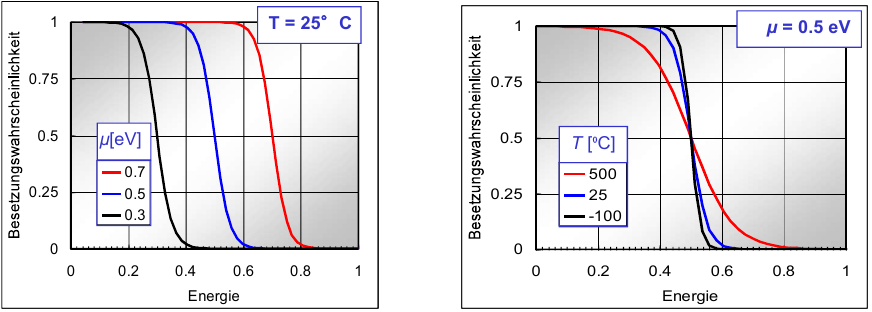
\includegraphics[width=\textwidth]{Kapitel/Kap04/fermiVerteilung.png}
			\caption{graphische Darstellung der Fermi-Verteilung}
			\label{04_fermiVert}
		\end{figure}
		(Besonders Temperaturabhängigkeit wichtig!)
		
	\subsubsection{Definition der Fermi-Energie}
		Fermi-Energie: $F_n = F_p = 0.5$
		
	\subsubsection{Lage des Fermi-Niveaus (intrinsisch vs. dotiert)}
		In undotierten Halbleiter liegt die Fermi-Energie i der Mitte der Bandlücke:
		$E_F(intrinsisch) = E_i = \frac{E_g}{2}$	
		
		Für n-dotierte Halbleiter liegt das Ferminiveau oberhalb des intrinsischen Niveaus und für p-dotierte Halbleiter liegt das Ferminiveau unterhalb des intrinsischen Niveaus.
	
		\begin{figure}[h!]
			\centering
			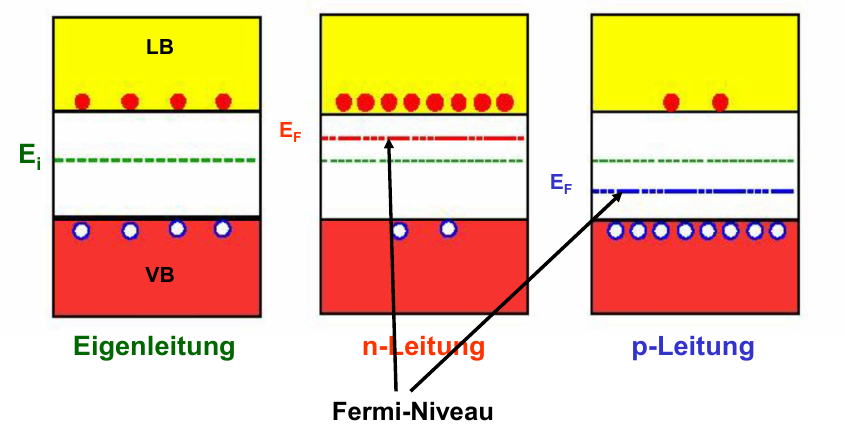
\includegraphics[width=0.6\textwidth]{Kapitel/Kap04/fermiNiveau.png}
			\caption{Fermi-Niveau eines undotierten, p-dotierten und n-dotierten HL}
			\label{04_fermiNiveau}
		\end{figure}
	
		\begin{figure}[h!]
			\centering
			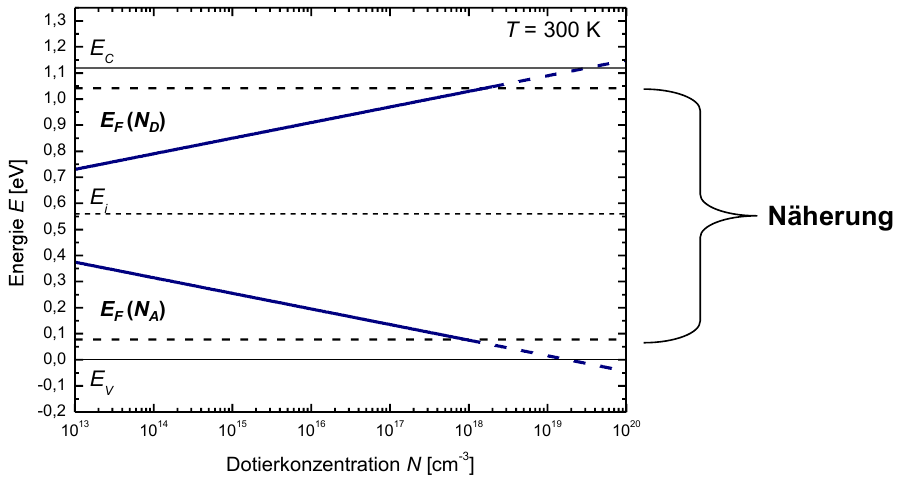
\includegraphics[width=0.8\textwidth]{Kapitel/Kap04/lageFerminiveauSi.png}
			\caption{Lage des Ferminiveaus bei steigender Dotierung}
			\label{04_lageFermiNiveau}
		\end{figure}
	
		\clearpage
			
		\begin{figure}[h!]
			\centering
			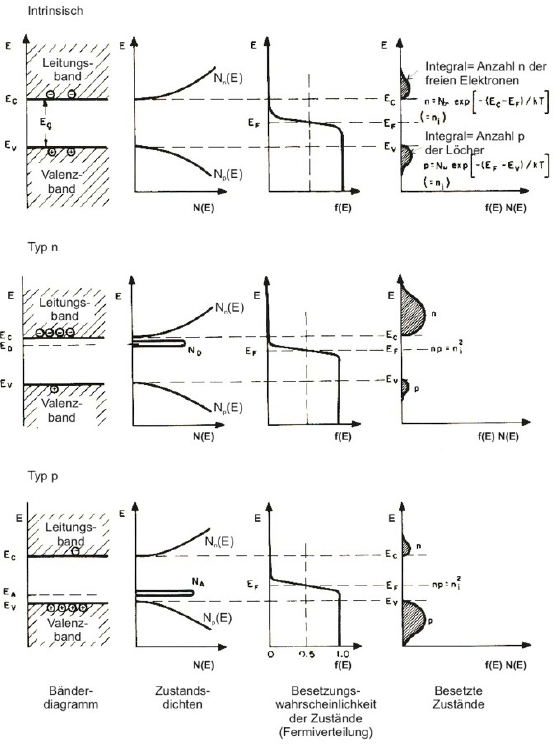
\includegraphics[width=0.6\textwidth]{Kapitel/Kap04/zustandsdichte.png}
			\caption{}
			\label{04_zustandsdichte}
		\end{figure}
		
			
	\subsubsection{Effektive Zustandsdichten}	
		%Die Zustandsdichte beinhaltet die Information über die Anzahl der Zustände, die im LB und VB besetzt werden können.
		%Bezeichnet als $D_n(E)$ wenn $E \geq E_{LB}$ und  $D_p(E)$ wenn $E \leq E_{VB}$.
		
		
\subsection{Ladungsträger im Halbleiter}
		
	\subsubsection{Massenwirkungsgesetz}
		Massewirkungsgesetz: $n \cdot p = {n_i}^2$
		bestimmt das Verhältnis zwischen Elektronen- und Löcheranzahl und gilt auch in dotierten Halbleitern
	\subsubsection{Neutralitätsbedingung}
		Da dotierte Halbleiter nur neutrale Bausteine beinhalten, ist er in seiner Gesamtheit elelktrisch neutral.
		Folgende geladene Teilchen können existieren:
		\begin{description}
			\item[$\bullet$] Freie Elektronen ($n$)
			\item[$\bullet$] Freie Löcher ($p$)
			\item[$\bullet$] Ionisierte Donatoren (${N_D}^+$)
			\item[$\bullet$] Ionisierte Akzeptoren (${N_A}^-$)
		\end{description}
		\textbf{Neutralitätsbedingung:}\\
		Bei dotierten Halbleitern gilt:\\
		$p + {N_D}^+ = n + {N_A}^-$\\
		
		(Bei Eigenleitung galt: Anzahl Elektronen = Anzahl Löcher)\\
		
		Bei vollständiger Ionisation (Störstellenerschöpfung):\\
		$n = N_D$ $p = N_A$ ${N_A}^- = N_A$ ${N_D}^+ = N_D$\\
		$\rightarrow n + {N_A}^- = p + {N_D}^+ = N_D + N_A$
			
	
	\subsubsection{Intrinsische Ladungsträgerkonzentration}
		Elektronen und Löcher sind in gleicher Zahl vorhanden.
		$n = p = n_i$
	\subsubsection{Bezeichnung von dotierten Halbleitern}
	
	\subsubsection{Majoritäten und Minoritäten}
		\textbf{Bei einem n-dotierten Halbleiter gilt:}\\
		Durch die Dotierung mit Donatoren gibt es viel mehr freie Elektronen als Löcher.
		Die Elektronen werde als Majoritätsträger, die Löcher als Minoritätsträger bezeichnet.
		Bei Störstellenerschöpfung ist die Majoritätskonzentration \textbf{temperatur\textcolor{red}{un}abhängig} und die Minoritätskonzentration \textbf{temperaturabhängig}.
		
		\begin{figure}[h!]
			\centering
			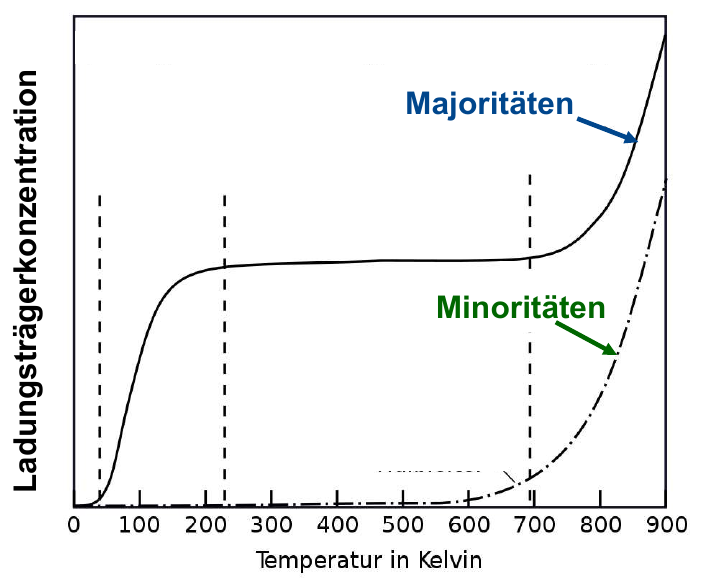
\includegraphics[width=0.6\textwidth]{Kapitel/Kap04/ladungstrKonzN.png}
			\caption{Temperaturabhängigkeit der Ladungsträgerkonzentration bei n-Dotierung}
			\label{04_ladungstrKonzN}
		\end{figure}
		\newpage
		
\subsection{Ladungsträgerbewegung}
	\begin{figure}[h!]
		\centering
		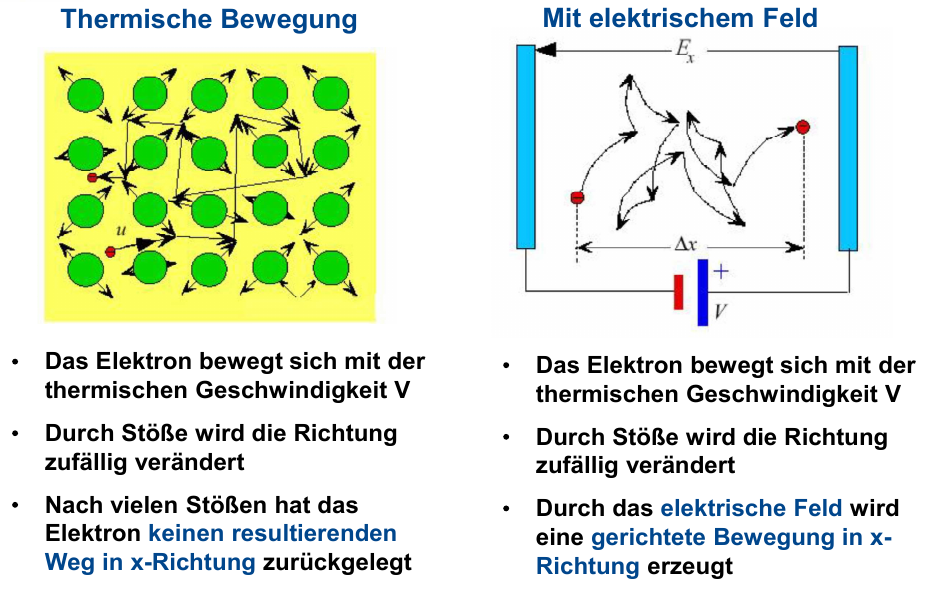
\includegraphics[width=0.6\textwidth]{Kapitel/Kap04/bewegungElektronen.png}
		\caption{Bewegung der Elektronen}
		\label{04_BewElek}
	\end{figure}
	
	\subsubsection{Driftstrom, Sättigung usw.}
		\textbf{Driftstrom:}
		Durch Stöße verlieren die Ladungsträger im Kristall immer wieder Energie (thermalisieren). $\rightarrow$ Es kommt (im Gegensatz zum Vakuum) nicht zur unbegrenzten Geschwindigkeitszunahme.
		Die Ladungsträger erreichen im Kristall eine mittlere endliche Geschwindigkeit , die \textbf{Driftgechwindigkeit $v_d$}.\\
		Unter dem Einfluss eines E-Feldes (Spannung) bewegen sich Löcher und Elektronen. Die Geschwindigkeit nimmt mit wachsendem Feld jedoch nicht stetig zu, sondern es tritt eine Sättigung ein. $\rightarrow$ Für kleine Feldstärken ist die Beweglichkeit eine Konstante, für größere Feldstärken nimmt die Beweglichkeit ab und erreicht einen Sättigungswert.
		
		\begin{figure}[h!]
			\centering
			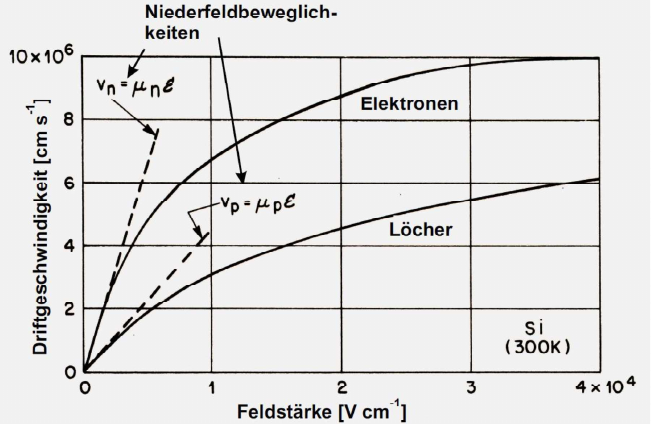
\includegraphics[width=0.6\textwidth]{Kapitel/Kap04/driftgeschwindigkeit.png}
			\caption{Driftgschwindigkeit}
			\label{04_driftGeschw}
		\end{figure}
		
		Zusammenhang zwischen Strom und Feld:\\
		\begin{equation*}
			\vec{E}_{el} \sim \vec{J}_{drift}
		\end{equation*}
		
		und
		
		\begin{equation}
			\vec{J}_{drift} = \vec{J}_{n/drift} + \vec{J}_{p/drift}
		\end{equation}
		wobei $\vec{J}$ die Teilchenstromdichte ist, dessen Betrag die Anzahl der Teilchen darstellt, die in der Sekunde durch die Flächeneinheit treten.
		
	\subsubsection{Diffusionsstrom und Temperaturspannung}
		Diffusion findet immer statt, wenn die Konzentration eines Stoffes von Ort zu Ort verschieden ist. Beendet wirde der Prozess erst durch völligen Ausgleich aller Konzentrationen (falls keine Quellen vorhanden sind). Der Teilchentransport wird durch den Gradienten der Teilchenzahl (Konzentration) angetrieben. Die Teilchenstromdichte $\vec{J}$ ist proportional zu dem Konzentrationsgefälle: $\vec{J} \sim grad(C)$ ($C$ = Konzentration).
		Diffusion und Beweglichkeit sind proportional zueinander (bei Elektronen und Löchern): $D \sim \mu$ .\\
		Der Quotient ist für Löcher und Elektronen in einem Material gleich: $\frac{D_p}{{\mu}_p} = \frac{D_n}{{\mu}_n} = U_T$ , und ist auch gleich der Temperaturspannung $U_T$.
			
\subsection{Leitfähigkeit von Halbleitern}
	Streuung an Dotierionen reduziert die mittlere Flugzeit und damit die Beweglichkeit. $\rightarrow$ die Beweglichkeit nimmt steigendem Dotierniveau ab.
	ei geringen Dotierstoffkonzentrationen dominiert die Streuung an den Gitterschwingungen (Phononen). Ab einer Dotierstoffkonzentration von mehr als $10^{15} cm^{-3}$ nimmt die Beweglichkeit stetig ab, jetzt dominiert die Coulombstreuung an den Ionen der Dotieratome.
	
	\begin{figure}[h!]
		\centering
		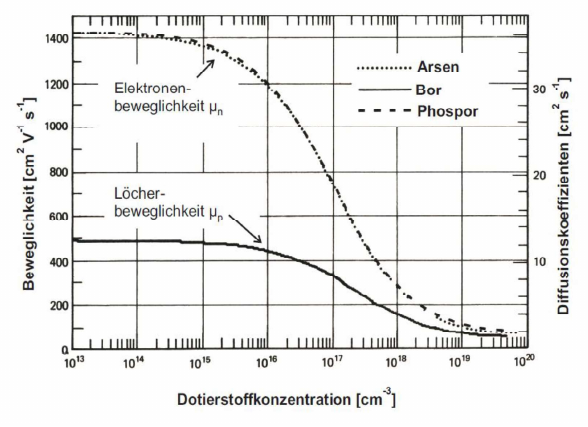
\includegraphics[width=0.6\textwidth]{Kapitel/Kap04/beweglichkeitKonzentration.png}
		\caption{Löcher und Elektronen in Silizium}
		\label{04_beweglKonz}
	\end{figure}
	
	\textbf{Driftstrom und Diffusionsstrom kompensieren sich $\rightarrow$ der Nettostrom ist gleich Null.}
	
	\subsubsection{p- und n-Typ, Temperaturabhängigkeit usw.}
		Bei gleichen Dotierniveaus haben p- und n-Silizium unterschiedliche Widerstände.
		
		\begin{figure}[h!]
			\centering
			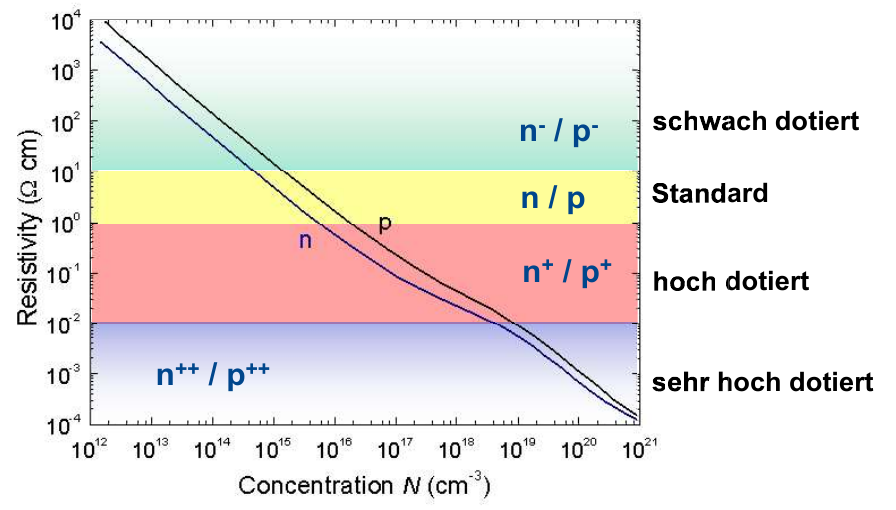
\includegraphics[width=0.6\textwidth]{Kapitel/Kap04/dotierungSi.png}
			\caption{Dotierungen von Silizium}
			\label{04_dotSi}
		\end{figure}
		
		\textbf{Temperaturabhängigkeit:}
		Bei hohen Temperaturen dominiert die Streuung an Phononen: $\mu \sim T^{-\frac{3}{2}}$ .\\
		Bei tiefen Temperaturen dominiert die Streuung an Störstellen: $\mu \sim T^{\frac{3}{2}}$ .\\
		\begin{figure}[h!]
			\centering
			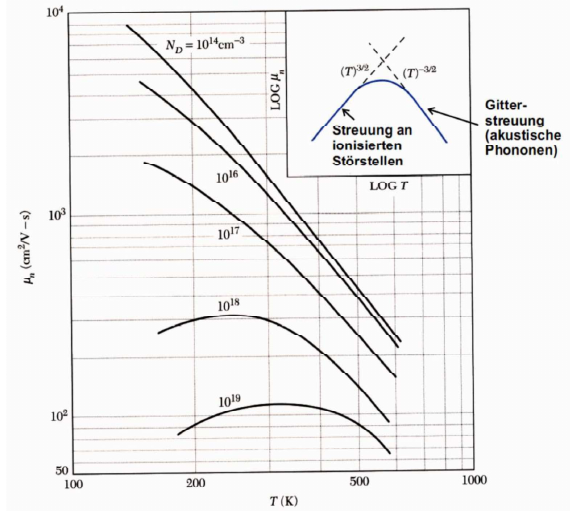
\includegraphics[width=0.6\textwidth]{Kapitel/Kap04/beweglInSi.png}
			\caption{Beweglichkeiten in Si}
			\label{04_beweglInSi}
		\end{figure}
		
	\subsubsection{Zusammenhang Ladungsträgerkonzentration intrinsisch und dotiert}
		
		\begin{figure}[h!]
			\centering
			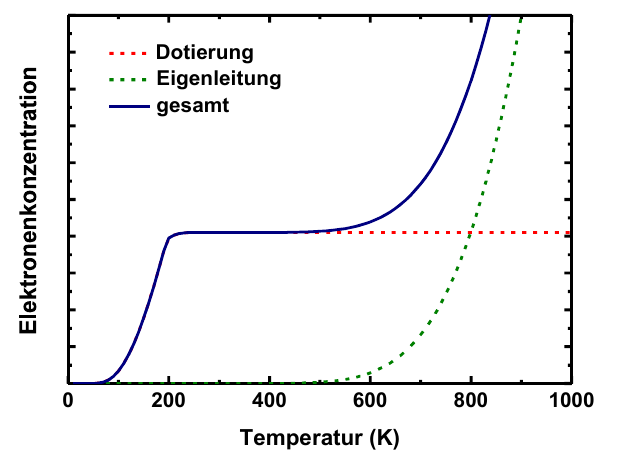
\includegraphics[width=0.6\textwidth]{Kapitel/Kap04/ladungstraegerKonz.png}
			\caption{Ladungsträgerkonzentration}
			\label{04_ladKonz}
		\end{figure}
	
		
	\subsubsection{Definitionen von Dotierniveaus}



\todo{Fragen aus Own Clowd zuordnen}
\todo{Gruppenübungs-Inhalte ergänzen}